\lecture{Thu. 10/4/12}

Last time we saw
\begin{itemize}
\item
$A_{TM}$ is undecidable.
\item
$\ol{A_{TM}}$ is T-unrecognizable.
\item 
Diagonalization method
\end{itemize}
We showed how the diagonalization method proved the reals were uncountable, and also applied the same idea to decidability. We'll give a quick recap, and highlight why the idea behind the two diagaonalization arguments are the same.
%Zack Remscrim
\begin{thm}
$\R$ is uncountable.
\end{thm}
\begin{proof}
Assume for contradiction that $\R$ is countable.
%Hilbert: is there intermediate infinitely (Hilbert's first problem).
%infinity is a basic notion in math
%something we want to understand if we can
%basic math question about nature of sets
%Gerdel, Paul Cohen l60s-e70s. Question not solvable using basic axioms of mathematics. Don't settle question one way or other. Unresolvable question.
Suppose we're given a bijection.

\begin{center}
\begin{tabular}{c|c}
$n$ & $f(n)$\tabularnewline
\hline 
1 & $2.71828\ldots$\tabularnewline
2 & $3.14159\ldots$\tabularnewline
3 & $0.11111\ldots$\tabularnewline
4 & $\vdots$\tabularnewline
$\vdots$ & $\vdots$\tabularnewline
\end{tabular}
\end{center}

Take a number differing from $f(i)$ in $i$th place. For instance, take $x=0.654\ldots$ where $6\ne 7$, $5\ne 4$, and $4\ne 1$.

Then $x$ can't be on the list. For instance, it can't be the 17th number because it's different in 17th place. Thus $f$ fails to be a bijection. This is Cantor's proof.
\end{proof}

We applied diagonalization to decidability problems.
\begin{thm}
$A_{TM}$ is undecidable.
\end{thm}
\begin{proof}
Assume $A$ is decidable by a Turing machine $H$.
Use $H$ to get TM $D$, that does the following.
\begin{enumerate}
\item
$D$ on $\an{M}$ rejects if $M$ accepts $\an{M}$ and accepts if $M$ rejects (halt or loop) $\an{M}$.
\end{enumerate}
Then $D$ accepts $\an{M}$ iff $M$ doesn't accept $\an{M}$; hence $D$ accepts $\an{D}$ if $D$ doesn't accept $\an{D}$, contradiction. 

This is the same idea as Cantor's diagonalization argument! To see this, let's make a table of how Turing machines respond to descriptions of Turing machines as inputs:

\begin{center}
\begin{tabular}{c|c|c|c|c|c|}
 & $\an{M_{1}}$ & $\an{M_{2}}$ & $\an{M_{3}}$ & $\cdots$ & $\an{D}$\tabularnewline
\hline 
$M_{1}$ &{\color{red} accept} & reject & reject & $\cdots$ & \tabularnewline
\hline 
$M_{2}$ & reject & {\color{red}reject} & reject &  & \tabularnewline
\hline 
$M_{3}$ & accept & accept &{\color{red}accept} & $\cdots$ & \tabularnewline
\hline 
$\vdots$ &  & $\vdots$ &  & $\ddots$ & \tabularnewline
\hline 
$D$ & rejects & accept & reject &  & ?\tabularnewline
\hline 
\end{tabular}
\end{center}

We programmed $D$ so that it differed from what $M_i$ decided on $\an{M_i}$. However we get a contradiction because nothing can go in the box labeled ``?", hence $D$ can't be on the list of all Turing machines.
%Method is the same! \fixme{Explain the diagram}
\end{proof}

Today we'll show a lot of other problems are undecidable. There's now a shortcut: by proving that $A_{TM}$ is undecidable, we will show a lot of other problems inherent $A_{TM}$'s undecidability. Then we won't need the diagonalization argument again. %Reducibility. Now and later on in complexity theory.

Today we'll use
\begin{enumerate}
\item
Reducibility to show undecidability
\item
Mapping reducibility to show T-unrecognizability.
\end{enumerate}
\subsection{Reducibility}
Let
\[
\text{HALT}_{TM}=\set{\an{M,w}}{\text{TM $M$ halts on input $w$}}.
\]
\begin{thm}\llabel{HALTTM}
$\text{HALT}_{TM}$ is undecidable.
\end{thm}
We can go back and use the diagaonlization method. But we'll give a different technique.
\begin{proof}
Suppose we can decide the halting problem by some Turing machine. We're going to use that to decide $A_{TM}$, which we know is not decidable. Hence our assumption that $\text{HALT}_{TM}$ is decidable must be false, i.e., the halting problem cannot be decided.

Assume for sake of contradiction that TM $R$ decides $\text{HALT}_{TM}$. We will construct a TM $S$ deciding $A_{\text{TM}}$.

%Pretend for the moment that someone gave you a $\text{HALT}_{TM}$ machine. %stayed up all night wrote a piece of java code miracle
%We'll show that can't be. We'll use that $\text{HALT}_{TM}$ decider to decide $A_{TM}$.
Let $S=$``on input $\an{M,w}$. 
\begin{enumerate}
\item
Use $R$ to test if $M$ halts on $w$. If not, reject. %(If $M$ doesn't halt on $w$, then we know $M$ rejects $w$.) 
If yes, run $M$ on $w$ until it halts." %Either way, we get an answer after finite time."
\end{enumerate}
Why does this work?
%Feed $M$ into $w$. 
If $M$ doesn't halt on $w$, %you feel good
then we know $M$ doesn't accept, so reject. %M doens't even halt -> answer doesn't accept.

Suppose $R$ says $M$ does halt. We don't know whether it accepts right off. Our algorithm says to run $M$ on $w$. We don't have to worry about $M$ going forever, because $R$ has told us that $M$ halts! We'll eventually come to the end, $M$ will accept or reject, and we can give our answer about $A_{\text{TM}}$.


Thus we can use our $\text{HALT}_{\text{TM}}$ machine to decide $A_{\text{TM}}$.
\end{proof}
This is called \textbf{reducing} $A_{TM}$ to the $\text{HALT}_{TM}$ problem.\\

\cpbox{\textbf{Reducibility}: One way to show a problem is undecidable is by reducing it from a problem we already know is undecidable, such as $A_{\text{TM}}$.\\

Concretely, to show a problem $P_1$ is undecidable, suppose it had a decider. Use the decider for $P_1$ to decide an undecidable problem (e.g. $A_{\text{TM}}$). This gives a contradiction.}
\vskip0.15in
If some problem has already been solved, and we reduce a new problem to an old problem, then we've solved it too. For instance, consider the acceptance problem for DFA's. We showed that $A_{DFA}$ is decidable (Theorem~\ref{ADFA}). Then it immediately follows that $A_{NFA}$ is decidable, because we can reduce the $A_{NFA}$ problem to a $A_{DFA}$ problem (Theorem~\ref{ANFA}). We converted the new problem into the solved problem.

\begin{df}
We say $A$ is \textbf{reducible} to $B$ if a solution to $B$ gives a solution to $A$.
\end{df}
Here we used reducibility in a twisted way. If $A$ is reducible to $B$, we know that if we can solve $B$ then we can solve $A$. Hence if we can't solve $A$ then we can't solve $B$.

%Means if we cannot solve $A$, then we cannot solve $B$.

We used a $\text{HALT}_{TM}$ machine to decide $A_{TM}$, so we reduced $A_{TM}$ to $\text{HALT}_{TM}$.

All ``natural" problems which are undecidable can be shown to be undecidable by reducing $A_{TM}$ to them or their complement.\\
%Can construct other pathological examples can't construct $A_{TM}$. 

%theory of structure of turing degrees.

\wrbox{
When trying to show problems are undecidable, reduce {\it from} $A_{TM}$ (not to $A_{TM}$).\footnote{On an undecidability problem on the exam, if you just write ``reduction from $A_{TM}$" you will get partial credit. If you write ``reduction to $A_{TM}$" you will get less credit.}}
\vskip0.15in
%solution to B yields solution to A: different, sharper requirement. Vague. What does solution mean? Prototype example. Precise by solvable.
%Turing machine.

Let
\[
E_{\text{TM}}=\set{\an{M}}{\text{TM }M\text{ and }L(M)=\phi}.
\]
\begin{thm}\llabel{thm:etm}
$E_{TM}$ is undecidable.
\end{thm}
\begin{proof}
Use reduction {\it from} $A_{TM}$ {\it to} $E_{TM}$. %(not other way around) %you lose points, I just erase

Here's the idea. Assume $R$ decides $E_{TM}$. We construct $S$ deciding $A_{TM}$. 
%Take inputs of the form $M$
%S can use $M$
%test whether M's language empty.
How do we do this? $S$ wants to decide whether a certain string is accepted; $R$ only tells whether the entire language is empty.
%If $M$'s language is empty, then reject because $M$ cannot accept $w$. %that's not my job. All I know is not empty.
%less obvious.
We're going to trick $R$ into giving me the answer we're looking for. 

Instead of feeding the TM $M$ into $R$, we're going to modify $M$. In the modified version of $M$ it's going to have $w$ built in: $M_w$. When start up $M_w$ on any input it will ignore that input, and just run $M$ on $w$. It doesn't matter what I feed it; it will run as if the input were $w$. The first thing it does is erase the input and writes $w$. $M_w$ will always to do the same thing: always accept or always reject, depending on what $M$ does to $w$. (The language is everything or nothing.) %find out whether M accepts w.

Now we feed $M_w$ into $R$. The only way the language can be nonempty is if $M$ accepts $w$. We've forced $R$ to give us the answer we're looking for, i.e., we've converted acceptance into emptiness problem. Now we're ready to write out the proof.

$S=$``On input $\an{M,w}$,
\begin{enumerate}
\item Construct $M_w=$``ignore input. 
\begin{enumerate}
\item
Run $M$ on $w$.
\item
\ul{Accept} if $M$ accepts."
\end{enumerate}
\item
Run $R$ on $\an{M_w}$.
\item
Give opposite answer.
($R$ is a decider. If $R$ accepts $\an{M_w}$, then $M_w$'s language is empty, so $M$ did not accept $w$, so reject.)
%reduce a_tm to math statement true of false 
\end{enumerate}
This machine decides $A_{\text{TM}}$, which is a contradiction. Hence our assumption was incorrect; $E_{\text{TM}}$ is undecidable.
\end{proof}
\subsection{Mapping reducibility}
We gave a general notion of reducibility, but not a specific definition. In this section we introduce a specific method called mapping reducibility.
\begin{df}
Let $A$ and $B$ be languages. We say that $A$ is \textbf{mapping reducible to} $B$, and write\footnote{Think of the notation as saying $A$ is ``easier" than $B$}
\[
A\le_m B
\]
if there is a \textbf{computable function} $f:\Si^*\to \Si^*$ and for all $w$, $w\in A$ iff $f(w)\in B$.

We say $f:\Si^*\to \Si^*$ is \textbf{computable} if some TM $F$ halts with $f(w)$ on the tape when started on input $w$.
%A function such that there is Turing machine that can output $f(w)$ when given the input $w$.
\end{df}

\begin{center}
\begin{figure}[h!]
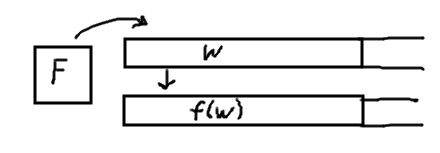
\includegraphics[scale=1.0]{9-1}
\qquad
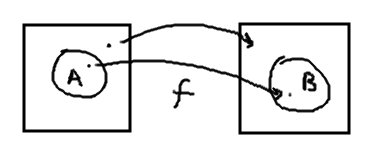
\includegraphics[scale=1.0]{9-2}
\end{figure}
\end{center}


Why is mapping reducibility useful? Suppose we have a decider for $B$, and we have $f$, computed by a decider. We can use the two deciders together to decide whether a string is in $A$!
%\begin{enumerate}
%\item
%Map the string by $f(w)$.
%\item Use the decider for $B$ to test if $f(w)$ is in $B$.
%\end{enumerate}
\begin{pr}\llabel{pr:map-reduce}
If $A\le_mB$ and $B$ is decidable (recognizable) so is $A$. %cell phone: thought that was me
\end{pr}
\begin{proof}
Say $R$ decides $B$. Let $S=$``On $w$,
\begin{enumerate}
\item
Compute $f(w)$.
\item 
Accept if $f(w)\in B$. 
Reject otherwise."
\end{enumerate}
For $B$ recognizable, just remove the last line ``reject if $f(w)\nin B$." (We don't know that $R$ halts.)
\end{proof}
Think of $f$ as a ``transformer": it transforms a problem in $A$ to a problem in $B$. If $A$ is reducible to $B$, and $A$ is not decidable, then neither is $B$.

This will also help us prove a problem is non-T-recognizable.

Let's recast our previous results in the language of mapping reducibility.

In the proof of Theorem~\ref{thm:etm} we showed that
\[
A_{TM}\le_m \ol{E_{TM}}.
\]
%cold chill
We converted a problem about $A_{TM}$ to a problem about $E_{TM}$. Given $\an{M,w}\in A_{TM}$, let $f$ map it to $\an{M_w}$. We have $\an{M,w}\in A_{TM}$ iff $M_w\nin E_{TM}$.
%not helpful look in other direction.

\ig{9-3}{1}

%complementations confusing.

%constructing specific examples on RHS. Only small set of machines in image. Doesn't make sense to reverse. Reduction another way is a different question.

A useful fact is that
\[
A\le_mB\iff \ol{A}\le_m \ol B;
\]
by using the same $f$.

We make one more observation, then prove another theorem.

We actually have the following strengthened version of Theorem~\ref{thm:etm}.
\begin{thm}\llabel{thm:etm2}
$E_{TM}$ is not recognizable.
\end{thm}
\begin{proof}
We showed $A_{TM}\le_m\ol{E_{TM}}$, so $\ol{A_{TM}}\le_m E_{TM}$. Since $\ol{A_{TM}}$ is not recognizable, $E_{\text{TM}}$ is not recognizable. %stronger property
\end{proof}

We'll now use mapping reducibility to give an example of a language such that neither it nor its complement is recognizable. %worst of both worlds
We will prove this by reduction from $A_{TM}$.
\begin{thm}\llabel{EQTM}
$EQ_{TM}$ and $\ol{EQ_{TM}}$ are both $T$-unrecognizable.
\end{thm}
Recall that the equality problem is that given 2 Turing machines, we want to know whether they recognize the same language. %Both problems are not recognizable. 
\begin{proof}
We show that
\begin{enumerate}
\item
$\ol{A_{TM}}\le_m EQ_{TM}$, or equivalently,
\[
A_{TM}\le_m \ol{EQ_{TM}}.
\]
We have to give a function \[
f:\an{M,w}\mapsto \an{M_1,M_2}.
\]
We let $M_2$ be the machine that always rejects. Let $M_1=M_w$, the machine that simulates $M$ on $w$. If $M$ accepts/rejects $w$ then the first will accept/reject everything and $M_2$ will reject everything, so $\an{M,w}\in A_{TM}$ iff $\an{M_1,M_2}\in \ol{EQ_{TM}}$.
\item
$\ol{A_{TM}}\le_m\ol{EQ_{TM}}$, or equivalently, 
\[
A_{TM}\le_mEQ_{TM}.
\]
We have to give a function \[
f:\an{M,w}\mapsto \an{M_1,M_2}.
\]
We let $M_2$ be the machine that always accepts. Again let $M_1=M_w$, the machine that simulates $M$ on $w$.
\end{enumerate}

\end{proof}

In the remaining 2 minutes, we'll look at a cool fact that we'll continue next time.

Lots of undecidable problems appear throughout math have nothing to do with Turing machines.

We'll give the simplest example. Let's define dominoes as pairs of strings of $a$'s and $b$'s, such as
\[
\bc{
\begin{bmatrix}
aba\\
ab
\end{bmatrix},
\begin{bmatrix}
aa\\
ab
\end{bmatrix},
\begin{bmatrix}
\phantom{aa}\\
\phantom{aa}
\end{bmatrix},\ldots
}
\]
Given a set of dominoes, can we construct a \textbf{match}, which is an ordering of dominoes such that the string along the top is the same as the string along the bottom? One little point: each domino can be reused as many times as we want. This means we have a potentially unlimited set of dominoes.

Is it possible to construct a match?

This is an undecidable problem!

And it has nothing to do with automata. But next time we will show we can reduce $A_{TM}$ to this problem; therefore it's undecidable.